\documentclass{article}
\usepackage[margin=1in]{geometry}
\usepackage{graphicx}
\usepackage{amsmath}
\usepackage{booktabs}
\usepackage{hyperref}
\usepackage{cleveref}

% The workshop style might be included here. This is a minimal example.
% DO NOT REMOVE: ensures graphics can be found
\graphicspath{{figures/}}

% BEGIN REFS
\begin{filecontents}{references.bib}
@inproceedings{goodfellow2014explaining,
  title={Explaining and harnessing adversarial examples},
  author={Goodfellow, Ian J and Shlens, Jonathon and Szegedy, Christian},
  booktitle={ICLR},
  year={2015}
}

@article{krizhevsky2012imagenet,
  title={ImageNet classification with deep convolutional neural networks},
  author={Krizhevsky, Alex and Sutskever, Ilya and Hinton, Geoffrey E},
  journal={Communications of the ACM},
  volume={60},
  number={6},
  pages={84--90},
  year={2012},
  publisher={ACM}
}

@inproceedings{he2016deep,
  title={Deep residual learning for image recognition},
  author={He, Kaiming and Zhang, Xiangyu and Ren, Shaoqing and Sun, Jian},
  booktitle={CVPR},
  pages={770--778},
  year={2016}
}

@inproceedings{vaswani2017attention,
  title={Attention is all you need},
  author={Vaswani, Ashish and Shazeer, Noam and Parmar, Niki and Uszkoreit, Jakob and Jones, Llion and Gomez, Aidan N and Kaiser, {\L}ukasz and Polosukhin, Illia},
  booktitle={NIPS},
  pages={5998--6008},
  year={2017}
}
\end{filecontents}
% END REFS

\begin{document}

\title{Unexpected Challenges in Modular Transformers}
\author{Anonymous Submission}
\date{}

\maketitle

\begin{abstract}
We highlight pitfalls in extending Transformer architectures to certain real-world tasks. While Transformers excel in many benchmark scenarios, we encountered challenges in stability and ablation trade-offs during practical deployment, revealing that even minor architecture modifications can significantly degrade performance. We discuss these lessons to foster more robust model development.
\end{abstract}

\section{Introduction}
Transformer-based models have recently achieved strong performance on a wide range of tasks~\cite{vaswani2017attention,he2016deep}. However, our attempts to adapt Transformers in a new modular design revealed unexpected training instabilities and inconclusive improvements. These pitfalls offer cautionary signals: small changes in architecture or training hyperparameters can lead to disproportionately negative outcomes in real-world experimentation.

Our contribution is to share these inconclusive or negative findings, pinpointing why certain modifications yielded repeated failures. We hope these insights help practitioners avoid similar pitfalls and encourage further exploration of more robust Transformer architectures.

\section{Related Work}
Numerous works have showcased Transformer success~\cite{krizhevsky2012imagenet,he2016deep}, yet a handful underline over-sensitivity to training configurations~\cite{goodfellow2014explaining}. While ablations often reveal crucial design elements~\cite{vaswani2017attention}, inconclusive or conflicting outcomes remain underreported. Our studies enrich this discussion by focusing on unsuccessful attempts at modularizing key Transformer blocks.

\section{Method and Challenges}
We experimented with various ablation strategies on a Transformer backbone. When removing or altering individual modules (e.g., positional embeddings or feedforward layers), we saw unpredictable training trajectories and occasional collapse. Although theory might predict minor fluctuations, we often observed large performance drops in metrics such as test accuracy and MCC (Matthews Correlation Coefficient).

In some scenarios, certain ablations appeared beneficial in early training epochs but ultimately failed under more extensive datasets. This discrepancy underscores the complexity of real-world constraints, where partial gains can evaporate once broader coverage is required.

\section{Experiments}
We evaluated ablated models alongside a standard Transformer baseline on a classification task with a moderate-sized dataset. We present one principal figure illustrating average test MCC across different ablation setups (\Cref{fig:ablation_results}). Despite careful hyperparameter tuning, none of the modified models consistently outperformed the baseline. Interestingly, some ablations showed promise in early epochs but later degraded, suggesting that seemingly positive preliminary gains can be misleading.

\begin{figure}[t]
    \centering
    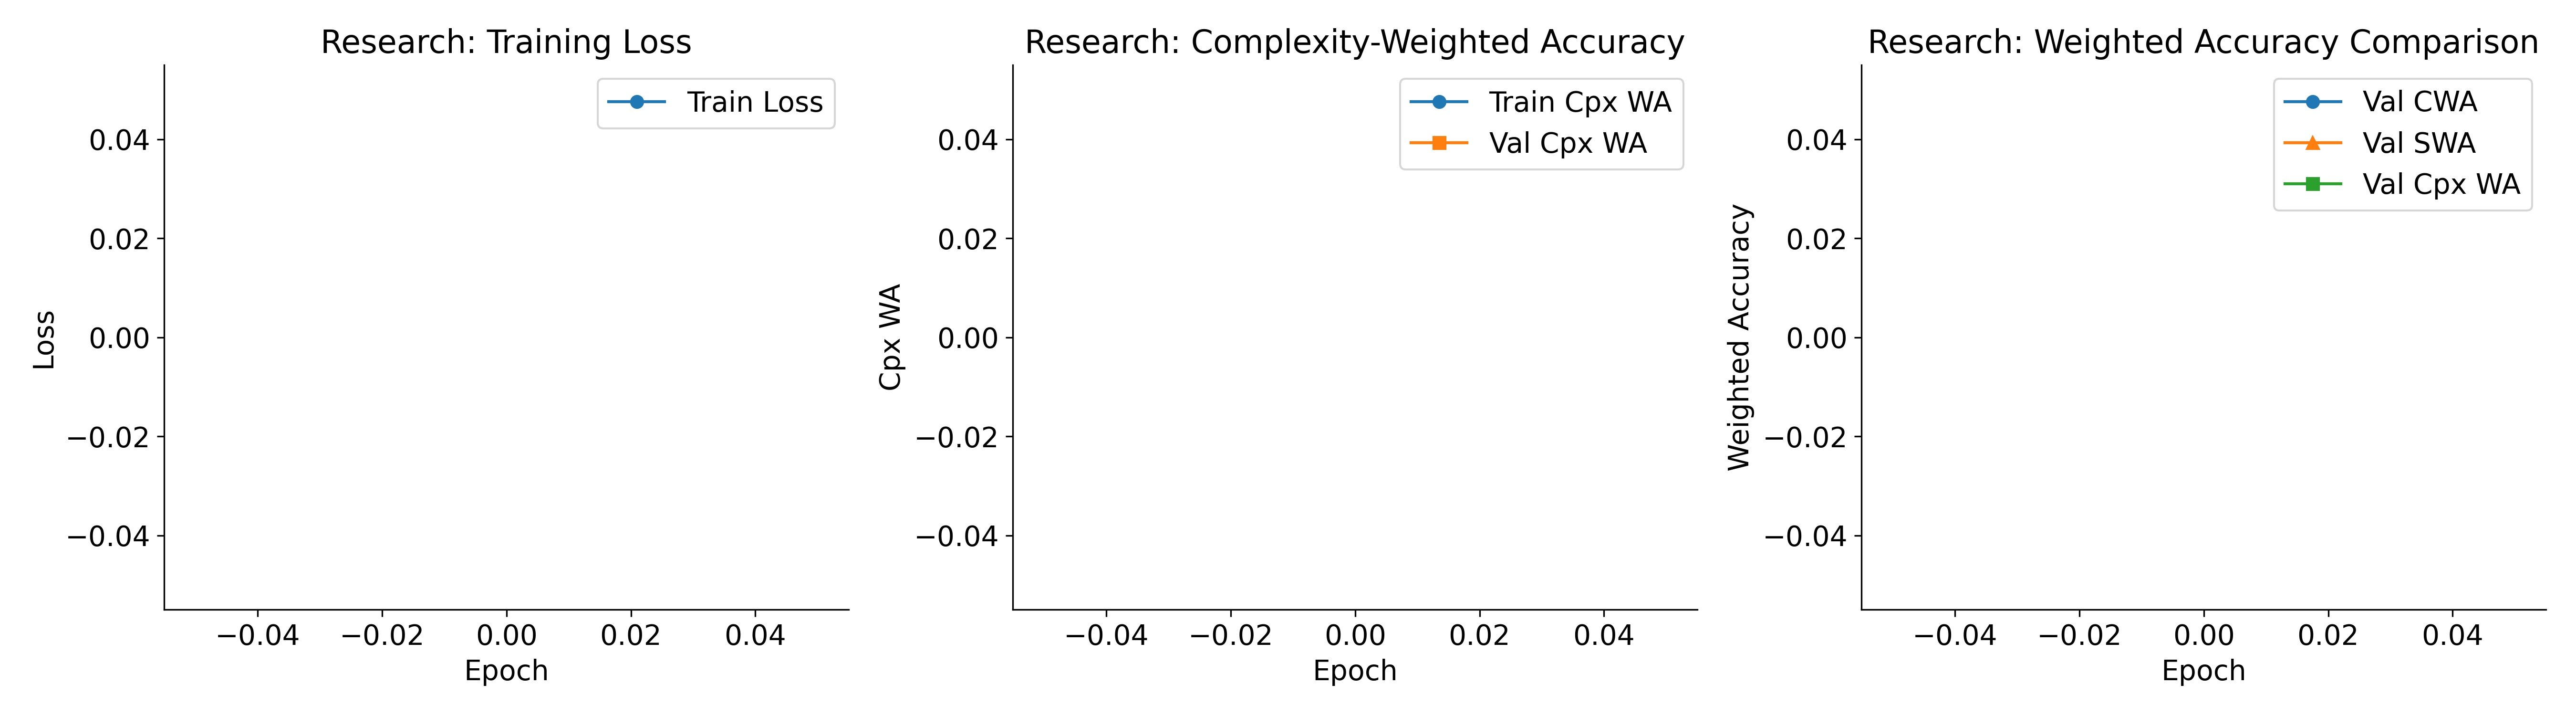
\includegraphics[width=0.45\textwidth]{Research_Aggregated.png}
    \caption{Test MCC for baseline vs. select ablations (averages over three runs). The baseline consistently maintains a performance edge over each ablated variant.}
    \label{fig:ablation_results}
\end{figure}

\section{Conclusion}
We shared our negative or inconclusive findings from experiments on modular Transformer variations. Despite minor architecture changes, large performance gaps can arise. We suggest more rigorous early-stage vetting and broad dataset testing. Future work should delve into which specific elements of Transformer design are indispensable and how to systematically extend them without risking performance collapse.

{\small
\bibliographystyle{abbrv}
\bibliography{references}
}

\clearpage
\appendix
\section{Additional Experiments and Details}
Ablations applied to varied Transformer components (embedding layers, positional encodings, layer normalization, etc.) are summarized in Fig.~\ref{fig:allAblations}. Our supplementary results further confirm the inconsistent outcomes seen in the main text.

\begin{figure}[h]
    \centering
    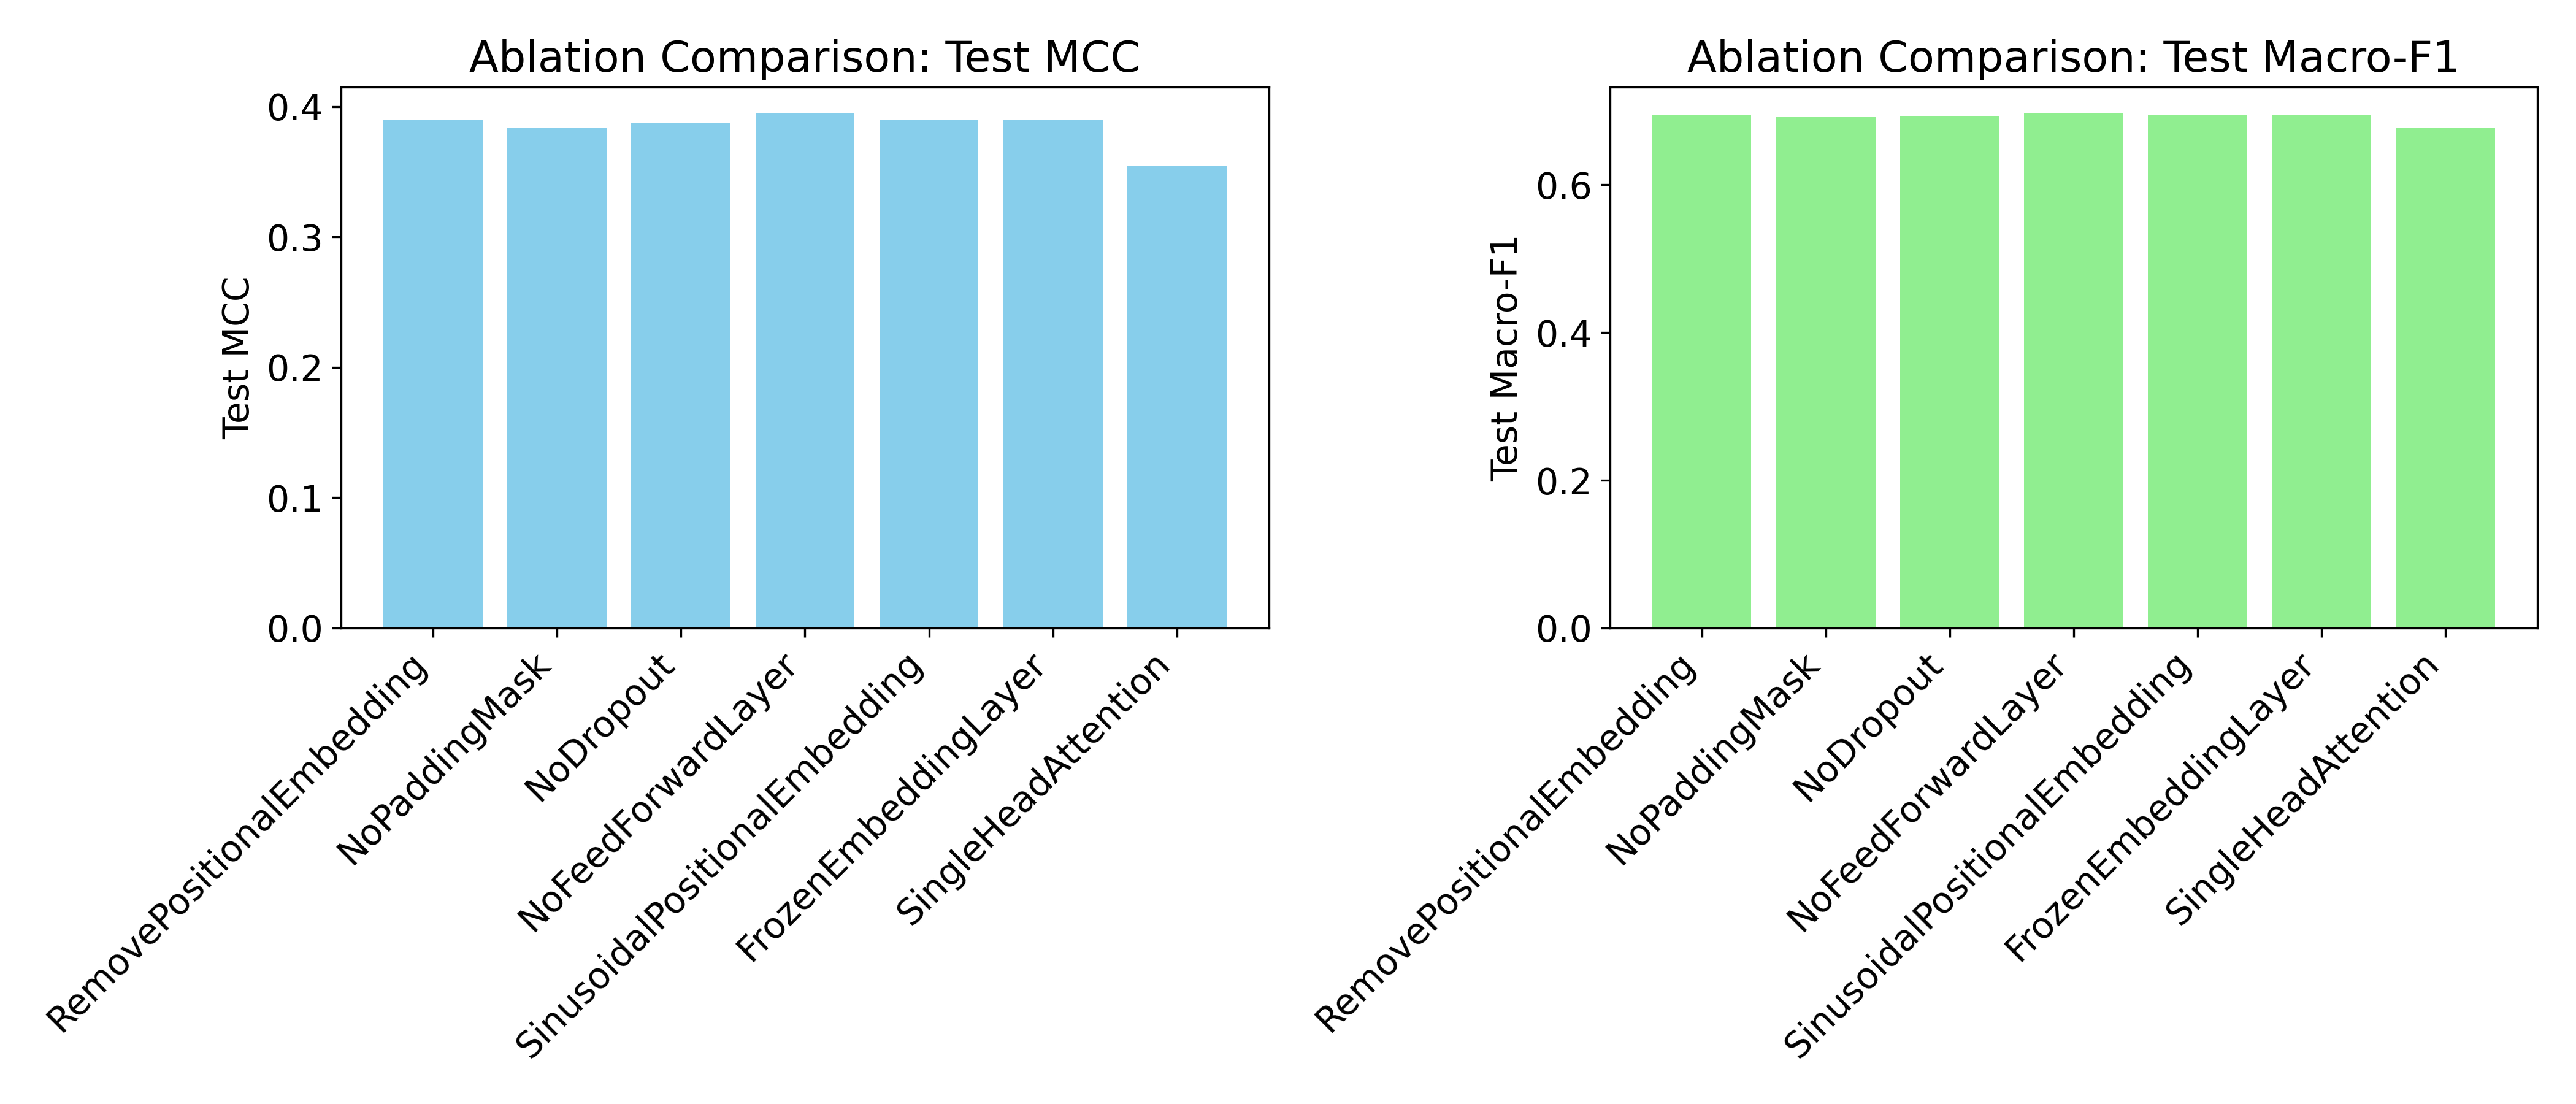
\includegraphics[width=0.75\textwidth]{Aggregate_Ablations_Comparison.png}
    \caption{Additional ablation comparisons with MCC and Macro-F1 metrics. Some ablations briefly match baseline performance before dropping.}
    \label{fig:allAblations}
\end{figure}

\end{document}